\title{Deploying CouchDB Cluster}


\author{Ribka Rufael}
\orcid{}
\affiliation{%
  \institution{School of Informatics and Computing}
  \streetaddress{}
  \city{Bloomington} 
  \state{IN} 
  \postcode{47408}
  \country{USA}
}
\email{rrufael@iu.edu}



% The default list of authors is too long for headers}
\renewcommand{\shortauthors}{R. Rufael}


\begin{abstract}
  This project focuses on deployment of CouchDB Cluster using Ansible
  playbook on Ubuntu Chameleon Cloud VMs and benchmarking of the
  deployment.
\end{abstract}

\keywords{hid-sp18-703, CouchDB}


\maketitle

\section{Introduction}

CouchDB~\cite{www-Couchdb} is a no sql database management system
under Apache. Data is stored as documents in CouchDB. In this project
CouchDB cluster of one or more Chameleon cloud VMs is deployed using
Ansible playbook and benchmarking is done to measure the time it took
for deployement using Bash scripts. After installation of CouchDB
cluster on Chameleon cloud VM, benchmarking test will be performed on
measuring write and read time on CouchDB database. The dataset which
was used for write and read on CouchDB is the wine quality dataset
from UCI Machine Learning Repository~\cite{www-WineQuality}.

\section{Ansible}
Ansible is a tool that help automate software deployments, system
configuration and continues deployment of applications. Automation
tasks are defined in Ansible Playbooks using YAML language. For
transportation, Ansible uses OpenSSH~\cite{www-Ansible}. 

For this project, Ansible was used to install CouchDB, configure
CouchDB in single node or cluster configuration and to create database
in CouchDB with different replication and sharding configurations on
Chameleon cloud VMs. 

\section{Chameleon Cloud}
The Chameleon project provides open and large scale platforms for
reaserchers. Chameleon project gets its funding from National Science
Foundation (NSF). Reaserchers will be able to investigate and come up
with solutions for problems in Software as a Service, Platforms as a
Service and vitual technologies. Both Bare metal and OpenStack Virtual
environements are available for researchers to use on Chameleon
project~\cite{www-Chameleon}. For this project, OpenStack virtual
machines were used and VM instance management was done through the
OpenStack web user interface~\cite{www-ChameleonDoc}. 

\section{Python}
Python programing language was used in this project to develop script
that was used for  preparing the test dataset with proper JSON format
used in CouchDB benchmarking process. Also python was used to develop
the script which is used in the analysis of the benchmark process outputs.

\section{CouchDB}
Apache CouchDB is an open source and NoSQL database system. In CouchDB
data is stored in documents. Documents in CouchDB have unique names, contain
metadata and content of the document is in semi structured JSON format. The fields in
the document can be different data types and there is no size
limit. Some of the supported data types for the content of documents
in CouchDB are strings, numbers, arrays, boolean and JSON
objects. There is no locking mechanism in CouchDB when adding,
updating or deleting documents. If two applications are making an
update to the same document in CouchDB database, upon save the
application has to resolve the conflict before merging the new
changes. Also while adding, updating or deleting documents in couchDB,
if the process fails before finishing then nothing gets saved in the
document. The update process has to finish successfully in order to
save the changes to the document. Read, write, update and delete
operations to CouchDB documents is done through RESTful
APIs. User can also interact with CouchDB through Fauxton which is
an administration user interface. Multi-Version Concurrency Control
(MVCC) is used as concurrency model in CouchDB. CouchDB uses views to
present structured data to users and applications. Views are
implemented in Javascript, use mapreduce model and are stored under
the design documents~\cite{www-Couchdb}. 

\subsection{Version}
The version of CouchDB used for this project is version 2.1.1 and this
is the current version at the time of writing this report.

\subsection{Architecture}
CouchDB 2.1.1 provides two setup configurations. These setup
configurations are single node and clustered configurations. As the
name suggests, CouchDB in single node configuration runs on a single
node. Whereas in clustered configuration CouchDB runs on multiple
nodes or servers~\cite{www-Couchdb, www-CouchdbOverview}.

\subsection{Security}
The ports that are used by CouchDB cluster are 5984 and 5986. Port
4369 is used by Erlang to identify the nodes in CouchDB cluster. Also
ports 9100-9200 for Erlang on different VMs to communicate to each
other. These ports should be opened to accept TCP protocol for all the
servers or VMs that are in the cluster~\cite{www-CouchdbSetup}. 
In the deployment for this project, security group rules were
created in Chameleon cloud which opened inbound TCP protocol for ports
5984, 5986 and 9100-9200.


\section{Deployment}
The deployment of CouchDB  was done through an automated Ansible
playbook. 
\subsection{Resource}
Table \ref{t:resource-specification} provides the specification for
the Chameleon Cloud Virtual Machines used in this project.

\begin{table}[]
\centering
\caption{Resource Specification}
\label{t:resource-specification}
\begin{tabular}{|l|l|l|l|l|l|}
\hline
\textbf{Instance} & \textbf{Image}       & \textbf{Size} & \textbf{RAM} & \textbf{VCPUs} & \textbf{Disk} \\ \hline
Node1             & Ubuntu16.04-20180205 & m1.medium     & 4GB          & 2              & 40GB          \\ \hline
Node2             & Ubuntu16.04-20180205 & m1.medium     & 4GB          & 2              & 40GB          \\ \hline
\end{tabular}
\end{table}

After starting two Instance  with the specification in Table
1~\ref{t:resource-specification}, allocating floating IPs to these 
instance and adding the security rules as mentioned under Security
section, user has to manually insert the IP addresses by modifying
inventory.txt file which is found under /project-code/couchdbansible
directory. 

\subsection{couchdbinstall.sh}

The bash script couchdbinstall.sh, takes three command line inputs
from the user. First parameter is tells the script whether to install
CouchDB in single node or cluster configuration. The second input the
number of replicas. The third input is the number of shards. An
example command looks like `./couchdbinstall.sh true 8 4` which
deploys CouchDB in cluster configuration and creates a database with 8
replicas and 4 shards.

The Ansible script that deploys CouchDB and it's dependencies are run
within couchdbinstall.sh. This script also creates csv file which
contains information about cluster setup, number of replicas, number
of shards and the time it took for couchDB install.

\subsection{Ansible Scripts}
All Ansible scripts reside under /project-code/couchdbansible
directory. 
\begin{enumerate}
  \item playbook.yml- defines the hosts on which CouchDB will be
    installed and the role name. This file along with inventory.txt is
    needed when runing Ansible playbook.

  \item main.yml-this file which is found under /roles/couchdb/tasks
    directory and this where all the installation tasks are
    defined. Some of the tasks defined are installation of Python
    pandas module since the VM in Chameleon did not have pandas
    installed, installation of CouchDB 2.1.1 and all it's dependencies
    and database creation after the installation of CouchDB.

  \item vmargs.j2- under /roles/couchdb/templates directory, template
    file that defines the CouchDB node names with the correct IP addresses.
\end{enumerate}

\subsection{Deploy Time}
The time taken for deployment of CouchDB on two Chameleon VMs was recorded for different
scenarios. As it can be seen in table~\ref{t:CouchDB-DeployTime},
CouchDB was installed in single node configuration/cluster configuration and different
number of replicas and shards. The first scenario which is basic installation of CouchDB
in single node configuration and no replicas and shards took 54 seconds
amount of time to finish. The sceond scenario, installation of CouchDB
in cluser configuration with two nodes configuration, 3 replicas and
8 shards took 52 seconds. The third scenario, installation of CouchDB
in cluser configuration with two nodes configuration, 4 replicas and
12 shards took 53 seconds. 

\begin{table}[]
\centering
\caption{CouchDB Deploy Time}
\label{t:CouchDB-DeployTime}
\begin{tabular}{|l|l|l|l|l|}
\hline
  & \textbf{Cluster\_Setup} & \textbf{replica\_val} & \textbf{shard\_val} & \textbf{Install time in seconds} \\ \hline
1 & False                   & 1                     & 1                   & 54                               \\ \hline
2 & True                    & 3                     & 8                   & 52                               \\ \hline
4 & True                    & 4                     & 12                  & 53                               \\ \hline
\end{tabular}
\end{table}

\section{Benchmark Results}
\subsection{Dataset}
The dataset that was used for the benchmarking process for this
project is the white vinho verde varient of Portuguese wine sample
from UCI Machine Learning Repository. The dataset was in CSV file
format and contains twelve different attributes related to wine such
as fixed acidity,pH, alcohol and quality~\cite{www-WineQuality}. 

Since CouchDB bulk load process only accepts file in proper JSON
format, \verb|csv_to_json.py| python script was used to
download the white wine dataset directly from UCI Machine Learning
Repository and convert the CSV file into JSON format by utilizing
pandas and urllib python modules.

\subsection{DatasetBulkLoadReadCouchDB.sh}
This is the script when executed, loads the JSON wine sample dataset
into CouchDB, performs simple read operation on the wine sample
dataset in CouchDB and mapreduce on the wine sample
dataset in CouchDB and measures the time taken for each operation.

\begin{enumerate}
  \item The first thing this script does is, it copies \verb|csv_to_json.py|
python script to the remote VM and executes this python script inorder
to generate the JSON wine dataset.
  \item CouchDB has \verb|/{db}/_bulk_docs|
endpoint that is used to create multiple documents with singe POST
request~\cite{www-CouchdbBulkApi}. DatasetBulkLoadReadCouchDB.sh loads JSON wine dataset
into CouchDB  'test' database using this POST call through curl command
and measures the time taken to finish the bulk document load.

  \item DatasetBulkLoadReadCouchDB.sh performs find document operation to find documents
from wine dataset which have quality greater than 3 and measures the time taken to finish this find
operation. This is accomplished by making POST call to
\verb|/{db}/_find| endpoint which returns documents that meet query criteria~\cite{www-CouchdbFind}.

  \item we wrote mapreduce function mapreducefun.js, which returns
    total number of rows from wine dataset which have quality greater than 3. This mapreduce
    function was uploaded to CouchDB design document to create view and GET call to
    \verb|/db/_design/design-doc/_view/view-name| was
    made~\cite{www-CouchdbView}. DatasetBulkLoadReadCouchDB.sh
    executes this mapreduce function on wine dataset in CouchDB and
    measures the time taken to finish execution of mapreduce.
  \item The final step in DatasetBulkLoadReadCouchDB.sh is to gather
    all the time duration from these mentioned operations and save
    into csv file.

\end{enumerate}

\subsection{Benchmark Result Analysis}
There were two aims of the benchmarking process for this project. One
of the aims of the benchmarking process was to find the impact of
number of shards on bulk documents load into CouchDB, find documents
operation and map reduce on documents in CouchDB. The second aim of
the process was to find the impact of number of replicas on bulk
documents load into CouchDB, find documents operation and map reduce
on documents in CouchDB. 

\subsubsection{Number of Shards Impact on Bulk Load}

Figure~\ref{f:shard-bulk} depicts the the impact of number of shards
on bulk load documents to couchDB time in seconds.
\begin{figure}[!ht]
  \centering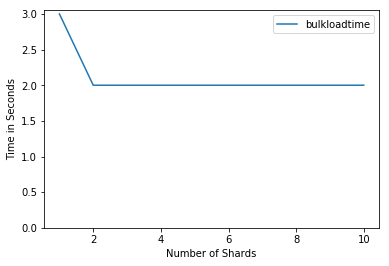
\includegraphics[width=\columnwidth]{../images/ShardsBulkLoad.png}
  \caption{Number of Shards vs Bulk Load Time in seconds }\label{f:shard-bulk}
\end{figure}



\subsubsection{Number of Shards Impact on Document Find}
\subsubsection{Number of Shards Impact on MapReduce}


\section{Conclusion}
TBD
\section*{Acknowledgements}

TBD

\bibliographystyle{ACM-Reference-Format}
\bibliography{report} 





